\documentclass[11pt]{article}
\usepackage[italian]{babel}
\usepackage{amsmath, amsfonts}
\usepackage{graphicx}
\begin{document}
\title{\Large Componenti connesse e albero di connessione minimo}\date{}
\author{Athos Innocenti}
\maketitle
\section{Introduzione}
In questa relazione vengono presentati l'algoritmo di Kruskal, per determinare l'albero di connessione minimo di un grafo non orientato, e l'algoritmo per trovare le componenti connesse di un grafo. Per poter eseguire entrambi gli algoritmi è stata implementata la struttura dati per insiemi disgiunti \textsc{Union-Find} con i relativi metodi \textsc{Union}, \textsc{Make-Set} e \textsc{Find-Set}.

Nell'analisi delle componenti connesse si valuta la relazione che sussiste tra l'aumento della probabilità di avere un arco tra due nodi del grafo e il numero di componenti connesse trovate.

Per l'algoritmo di Kruskal, invece, si valuta la relazione tra l'aumento della probabilità di avere un arco e il tempo di esecuzione dell'algoritmo. Inoltre, poiché l'albero di connessione minimo è un sottoinsieme aciclico di un grafo pesato non orientato che connette tutti i suoi nodi, sarà possibile eseguire l'algoritmo di Kruskal solo nel caso in cui il grafo in esame presenta una sola componente connessa. 
\section{Componenti connesse}
Una \textbf{componente connessa} di un grafo non orientato è una classe di equivalenza dei nodi secondo la relazione "è raggiungibile da". L'algoritmo per le componenti connesse usa le operazioni degli insiemi disgiunti per trovare le componenti connesse di un grafo. Inizialmente, la procedura pone ciascun vertice \textit{v} nel proprio insieme disgiunto. Poi, per ogni arco $(u,v)$, unisce gli insiemi che contengono i nodi \textit{u} e \textit{v}. Dopo che tutti gli archi sono stati esaminati, due nodi si troveranno nella stessa componente connessa, se e soltanto se i corrispondenti oggetti si trovano nello stesso insieme.
\subsection{Analisi dell'algoritmo per le componenti connesse}
Per poter analizzare l'algoritmo si considerano tre dimensioni del grafo casuale: un grafo con $25$ nodi, uno con $100$ e un terzo grafo avente $500$ nodi. La probabilità cresce da $0$ a $100$ per il grafo con $25$ nodi, da $0$ a $50$ per il grafo con $100$ nodi e da $0$ a $25$ per il grafo con $500$ nodi. Inoltre, per ciascun valore della probabilità vengono eseguite $10$ prove sulle quali viene fatta una media.

In riferimento ai grafici in figura \ref{cc25}, \ref{cc100} e \ref{cc500}, si nota che il numero di componenti connesse diminuisce velocemente all'aumentare della probabilità di avere archi. L'aumento della dimensione del grafo fa sì che il numero di componenti connesse tenda a $1$ in modo sempre più repentino: nel grafo con $25$ nodi già per valori della probabilità prossimi a $20$ il numero di componenti connesse è pressoché $1$ e via via che la dimensione aumenta si arriva ad ottenere un'unica componente connessa per valori della probabilità sempre più piccoli.
\begin{figure}[h]
\centering
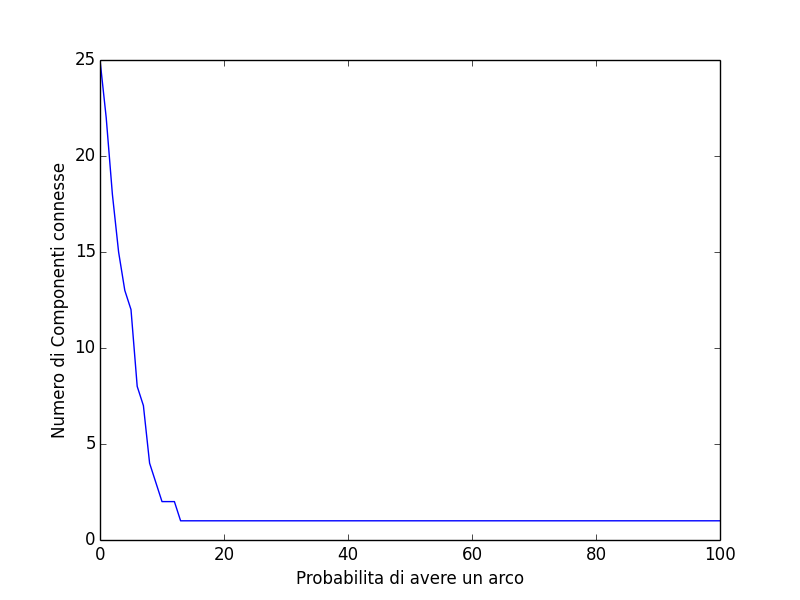
\includegraphics[scale=0.33,angle=0]{cc25.png}
\caption{Componenti connesse in un grafo di dimensione 25}
\label{cc25}
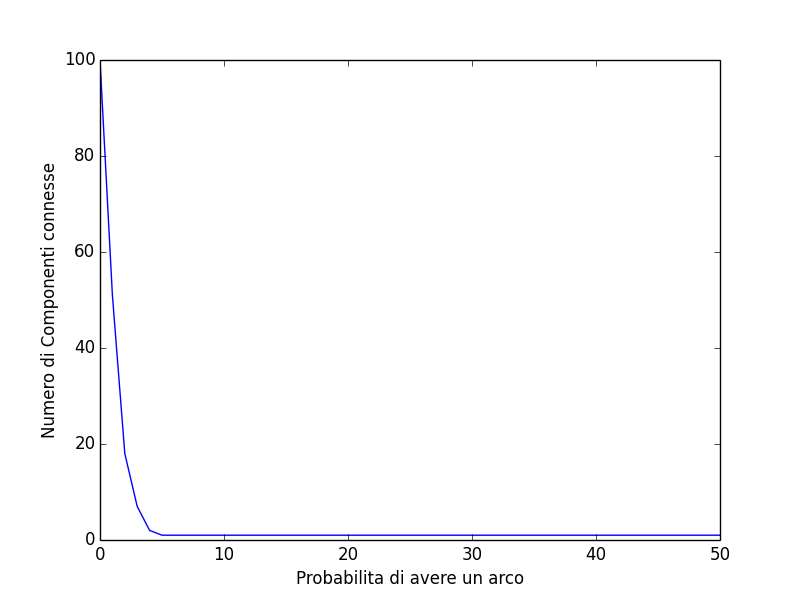
\includegraphics[scale=0.33,angle=0]{cc100.png}
\caption{Componenti connesse in un grafo di dimensione 100}
\label{cc100}
\end{figure}
\newpage
\begin{figure}[h]
\centering
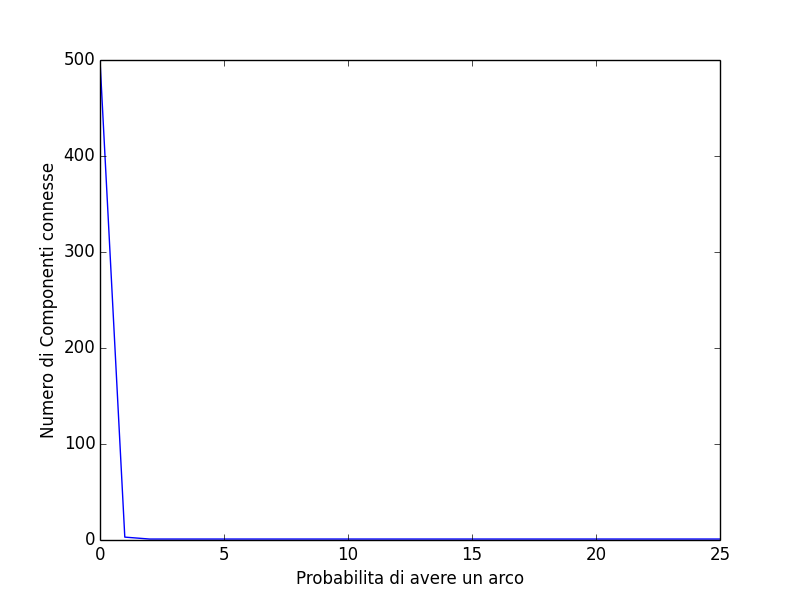
\includegraphics[scale=0.33,angle=0]{cc500.png}
\caption{Componenti connesse in un grafo di dimensione 500}
\label{cc500}
\end{figure}
\section{Alberi di connessione minimi}
Un \textbf{MST} o \textbf{albero di connessione minimo}, è un sottoinsieme aciclico di un grafo pesato non orientato $G = (V,E)$ che connette tutti i nodi del grafo e avente, per definizione, peso totale minimo. Tra gli algoritmi che consentono di determinare l'albero di connessione minimo di un grafo \textit{G} c'è l'algoritmo di Kruskal che implementa una strategia golosa.
\subsection{Algoritmo di Kruskal}
L'algoritmo di Kruskal, ad ogni passo, aggiunge ad un insieme \textit{A}, sottoinsieme di un qualche albero di connessione minimo e inizialmente vuoto, un arco sicuro $(u,v)$, ovvero un arco tale che l'insieme $A \cup \{(u,v)\}$ è ancora un sottoinsieme di un qualche MST. L'arco aggiunto è un arco di peso minimo nel grafo che collega due componenti distinte.

L'algoritmo di Kruskal è un algoritmo goloso, perché a ogni passo aggiunge alla foresta un arco con il minor peso possibile.

L'algoritmo, come detto, sfrutta le operazioni definite nella struttura dati \textsc{Union-Find} e il suo tempo di esecuzione è funzione sia del numero di nodi che del numero di archi del grafo, in particolare $T(n) = O(E\,lg\,V)$.
\subsubsection{Analisi dell'algoritmo di Kruskal}
Analogamente all'analisi dell'algoritmo per le componenti connesse, anche per l'analisi di Kruskal si considera un grafo casuale con $25$, $100$ e $500$ nodi. La probabilità cresce secondo lo stesso criterio utilizzato nell'analisi dell'algoritmo per le componenti connesse, eseguendo $10$ prove per ciascun valore, sulle quali viene fatta una media.

Come è possibile vedere dai grafici in figura \ref{k25}, \ref{k100} e \ref{k500} e dalla tabella \ref{t_k500}, all'aumentare della probabilità di avere archi corrisponde un incremento del tempo di esecuzione dell'algoritmo secondo un andamento approssimabile ad un logaritmo.
\begin{figure}[h]
\centering
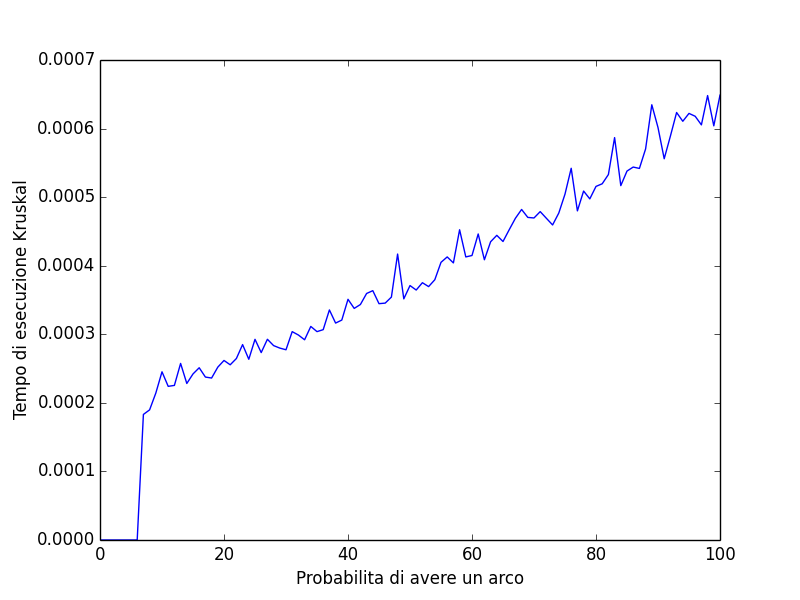
\includegraphics[scale=0.33,angle=0]{kruskal25.png}
\caption{Tempo di esecuzione di Kruskal in funzione della probabilità in un grafo di dimensione 25}
\label{k25}
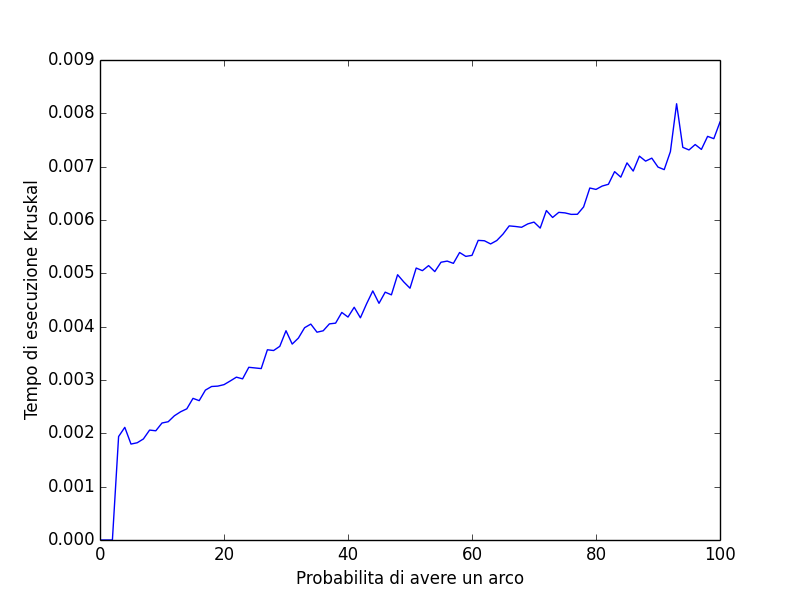
\includegraphics[scale=0.33,angle=0]{kruskal100.png}
\caption{Tempo di esecuzione di Kruskal in funzione della probabilità in un grafo di dimensione 100}
\label{k100}
\end{figure}
\newpage
\begin{figure}[h]
\centering
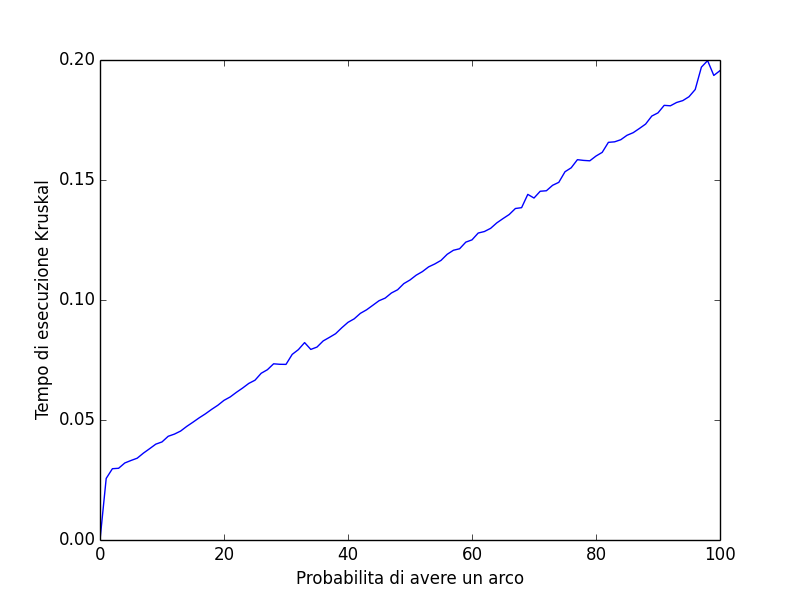
\includegraphics[scale=0.33,angle=0]{kruskal500.png}
\caption{Tempo di esecuzione di Kruskal in funzione della probabilità in un grafo di dimensione 500}
\label{k500}
\end{figure}
\begin{table}[h]
\centering
\begin{tabular}{|c|c|c|c|c|c|}\hline
Probabilità &20 &40 &60 &80 &100\\ \hline
Prova 1	&0.054	&0.086	&0.136	&0.203	&0.185 \\ \hline
Prova 2	&0.053	&0.085	&0.151	&0.161	&0.183 \\ \hline
Prova 3	&0.053	&0.115	 &0.141  &0.159	&0.195 \\ \hline
Prova 4	&0.055	&0.088	&0.158	&0.157	&0.196 \\ \hline
Prova 5	&0.067	&0.091	&0.197	&0.158	&0.198 \\ \hline
Prova 6	&0.054	&0.094	&0.151	&0.156	&0.204  \\ \hline
Prova 7	&0.054	&0.099	&0.146	&0.162	&0.193  \\ \hline
Prova 8	&0.054	&0.085	&0.173	&0.153	&0.189  \\ \hline
Prova 9	&0.054	&0.104	&0.149	&0.161	&0.193 \\ \hline
Prova 10	&0.055	&0.096	&0.139	&0.149	&0.191 \\ \hline
\end{tabular}
\caption{Tempi di esecuzione dell'algoritmo di Kruskal per un grafo di dimensione 500}
\label{t_k500}
\end{table}
\section{Conclusioni}
Tramite i dati ricavati dalle varie prove è possibile verificare come sia l'algoritmo per le componenti connesse che l'algoritmo di Kruskal siano entrambi influenzati dalla probabilità di avere archi nel grafo ma anche dalla dimensione del grafo stesso. Maggiore è la dimensione del grafo più velocemente il numero delle componenti connesse tenderà a 1 e maggiore sarà il tempo impiegato dall'algoritmo di Kruskal per trovare l'albero di connessione minimo.

I test sono stati eseguiti su un Macbook Pro con processore 2,7 GHz Intel Core i5, RAM 8 GB 1867 MHz DDR3 e sistema operativo macOS Mojave 10.14.6.
\end{document}